\appendix{Modules for Planar Pentagons}
\label{appPentagons}

There are three separate modules that collectively allow a description to be cast for a response of the twelve pentagons that comprise the surface of a dodecahedron.  The first module provides their shape functions.  The second module provides their kinematics, modeled as membranes.  While the third module incorporates these features into a viable description for pentagons.

\subsection{Shape Functions}
\label{appShapeFunctions}

Module \texttt{shapeFunctions} is Python code that exports class \texttt{shapeFunction}.  These shape functions are for the geometry of an irregular planar pentagon.  Shape functions for other geometries are not needed.  These objects are created within the \texttt{pentagon} constructor, and are utilized by the objects of that class.  Class \texttt{shapeFunction} has the following interface:

\medskip\noindent
\textbf{class} \texttt{shapeFunction}

\medskip\noindent
\textit{constructor}

\medskip\noindent
\texttt{sf = shapeFunction(xi, eta)} \\
\indent \texttt{xi} \;\;\;\: the $x$ co-ordinate in the natural co-ordinate system \\
\indent \texttt{eta} \;\;  the $y$ co-ordinate in the natural co-ordinate system

\medskip\noindent
where admissible co-ordinates \texttt{xi} and \texttt{eta} are any values that lie within the area of that pentagon which inscribes a unit circle or that reside along its boundary, as drawn in Fig.~\ref{figRegPentagon}.

\medskip\noindent
\textit{methods}

\medskip\noindent
\texttt{y = sf.interpolate(y1, y2, y3, y4, y5)}

\medskip\noindent
Returns an interpolation for field \texttt{y} at location (\texttt{xi, eta}) given values \texttt{y1, y2, y3, y4, y5} for some field of interest, which are evaluated at the five vertices of the pentagon, indexed according to Fig.~\ref{figRegPentagon}.  Arguments may be of any numeric type or that of a NumPy array.

\medskip\noindent
\texttt{Gmtx = sf.G(x1, x2, x3, x4, x5, x01, x02, x03, x04, x05)}

\medskip\noindent
Returns the displacement gradient 
\begin{displaymath}
   \mathbf{G} = \begin{bmatrix}
        \partial u / \partial x & \partial u / \partial y \\
        \partial v / \partial x & \partial v / \partial y 
   \end{bmatrix}
   \qquad \text{where} \qquad
   \begin{aligned}
        u & = x - X \\
        v & = y - Y
   \end{aligned}
\end{displaymath}
at that location with natural co-ordinates (\texttt{xi, eta}) residing within a pentagonal plane.  The arguments are tuples providing co-ordinate positions for the vertices of a pentagon in their pentagonal frame of reference, e.g., \texttt{x1} = ($x_1, y_1$), $\ldots$, \texttt{x01} = ($X_1, Y_1$), $\ldots$ with subscripts indexing according to Fig.~\ref{figRegPentagon}.

\medskip\noindent
\texttt{Fmtx = sf.F(x1, x2, x3, x4, x5, x01, x02, x03, x04, x05)}

\medskip\noindent
Returns the deformation gradient 
\begin{displaymath}
\mathbf{F} = \begin{bmatrix}
\partial x / \partial X & \partial x / \partial Y \\
\partial y / \partial X & \partial y / \partial Y 
\end{bmatrix}
\end{displaymath}
at that location with natural co-ordinates (\texttt{xi, eta}) residing within a pentagonal plane.  The arguments are tuples providing co-ordinate positions for the vertices of a pentagon in their pentagonal frame of reference, e.g., \texttt{x1} = ($x_1, y_1$), $\ldots$, \texttt{x01} = ($X_1, Y_1$), $\ldots$ with subscripts indexing according to Fig.~\ref{figRegPentagon}.

\medskip\noindent
\texttt{dFdXi = sf.dFdXi(x1, x2, x3, x4, x5, x01, x02, x03, x04, x05)}

\medskip\noindent
Returns the gradient of a deformation gradient taken with respect to the $\xi$ direction 
\begin{displaymath}
\frac{\partial\mathbf{F}}{\partial \xi} = \frac{\partial}{\partial \xi} 
\begin{bmatrix}
\partial x / \partial X & \partial x / \partial Y \\
\partial y / \partial X & \partial y / \partial Y 
\end{bmatrix}
\end{displaymath}
at that location with natural co-ordinates (\texttt{xi, eta}) residing within a pentagonal plane.  The arguments are tuples providing co-ordinate positions for the vertices of a pentagon in their pentagonal frame of reference, e.g., \texttt{x1} = ($x_1, y_1$), $\ldots$, \texttt{x01} = ($X_1, Y_1$), $\ldots$ with subscripts indexing according to Fig.~\ref{figRegPentagon}.

\medskip\noindent
\texttt{dFdEta = sf.dFdEta(x1, x2, x3, x4, x5, x01, x02, x03, x04, x05)}

\medskip\noindent
Returns the gradient of a deformation gradient taken with respect to the $\eta$ direction
\begin{displaymath}
\frac{\partial\mathbf{F}}{\partial \eta} = \frac{\partial}{\partial \eta} 
\begin{bmatrix}
\partial x / \partial X & \partial x / \partial Y \\
\partial y / \partial X & \partial y / \partial Y
\end{bmatrix}
\end{displaymath}
at that location with natural co-ordinates (\texttt{xi, eta}) residing within a pentagonal plane.  The arguments are tuples providing co-ordinate positions for the vertices of a pentagon in their pentagonal frame of reference, e.g., \texttt{x1} = ($x_1, y_1$), $\ldots$, \texttt{x01} = ($X_1, Y_1$), $\ldots$ with subscripts indexing according to Fig.~\ref{figRegPentagon}.


\subsection{Membranes}
\label{appMembranes}

Module \texttt{membranes.py} is Python code that exports class \texttt{membrane}.  Objects of this class are used to describe kinematic fields at the Gauss points of a pentagon.  These objects are created within the \texttt{pentagon} constructor, and are utilized by the objects of that class.  Class \texttt{membrane} has the following interface:

\medskip\noindent
\textbf{class} \texttt{membrane}

\medskip\noindent
\textit{constructor}

\medskip\noindent
\texttt{m = membrane(h)} \\
\indent \texttt{h} \;\; uniform time step separating any two neighboring configurations

\medskip\noindent
\textit{methods}

\medskip\noindent
\texttt{m.update(nextF)}
\medskip\noindent

Establishes the fields that pertain to this instance of \texttt{membrane} which affiliate with the deformation gradient \texttt{nextF} of the next configuration.  This is a $2 \times 2$ matrix describing the deformation gradient in the plane of the pentagon.  (It is not the deformation gradient sent to \texttt{d.update(nextF)} of \texttt{dodecahedron} objects.)  This method may be called multiple times before freezing its values with a call to \texttt{advance}.  (This method is called internally by \texttt{pentagon} objects.)

\medskip\noindent
\texttt{m.advance()}

\medskip\noindent
Assigns all of the object's data associated with the current configuration into their affiliated data associated with the previous configuration, and then assigns all of the object's data associated with the next configuration into their affiliated data associated with the current configuration, thereby freezing these data from external change.  (This method is called internally by \texttt{pentagon} objects.)

\medskip\noindent
\textit{Tensor fields that associate with a Gram-Schmidt factorization of the deformation gradient.}

\medskip\noindent
\texttt{qMtx = m.Q(state)}

\medskip\noindent
Returns the $2 \times 2$ re-indexing matrix that is applied to the deformation gradient prior to its Gram-Schmidt decomposition in configuration \texttt{state}.

\medskip\noindent
\texttt{rMtx = m.R(state)}

\medskip\noindent
Returns the $2 \times 2$ rotation matrix \textbf{Q} derived from a \textbf{QR} decomposition of the re-indexed deformation gradient in configuration \texttt{state}.

\medskip\noindent
\texttt{omega = m.spin(state)}

\medskip\noindent
Returns the $2 \times 2$ spin matrix caused by planar deformation, i.e., $\mathrm{d} \mathbf{R} \, \mathbf{R}^{\mathsf{T}}$, in configuration \texttt{state}.

\medskip\noindent
\texttt{uMtx = m.U(state)}

\medskip\noindent
Returns the $2 \times 2$ Laplace stretch \textbf{R} (denoted herein as $\boldsymbol{\mathcal{U}}$) derived from a \textbf{QR} decomposition of the re-indexed deformation gradient in configuration \texttt{state}.

\medskip\noindent
\texttt{uInvMtx = m.UInv(state)}

\medskip\noindent
Returns the $2 \times 2$ inverse Laplace stretch \textbf{R} (denoted herein as $\boldsymbol{\mathcal{U}}^{-1}$) derived from a \textbf{QR} decomposition of the re-indexed deformation gradient in configuration \texttt{state}.

\medskip\noindent
\texttt{duMtx = m.dU(state)}

\medskip\noindent
Returns the differential change of the Laplace stretch \textbf{R} derived from a \textbf{QR} decomposition of the re-indexed deformation gradient in configuration \texttt{state}.

\medskip\noindent
\texttt{duInvMtx = m.dUInv(state)}

\medskip\noindent
Returns the differential change of the inverse Laplace stretch \textbf{R} derived from a \textbf{QR} decomposition of the re-indexed deformation gradient in configuration \texttt{state}.

\medskip\noindent
\textit{Scalar attributes that arise as extensive thermodynamic variables.}

\medskip\noindent
\texttt{xi = m.dilation(state)}

\medskip\noindent
Returns the planar dilation derived from a \textbf{QR} decomposition of the re-indexed deformation gradient in configuration \texttt{state}, i.e., $\xi = \ln \sqrt{A / \! A_0}$.

\newpage
\medskip\noindent
\texttt{epsilon = m.squeeze(state)}

\medskip\noindent
Returns the in-plane squeeze derived from a \textbf{QR} decomposition of the re-indexed deformation gradient in configuration \texttt{state}, i.e., $\varepsilon = \ln \sqrt{ \Gamma \! / \Gamma_0}$.

\medskip\noindent
\texttt{gamma = m.shear(state)}

\medskip\noindent
Returns the in-plane shear derived from a \textbf{QR} decomposition of the re-indexed deformation gradient in configuration \texttt{state}.

\medskip\noindent
\texttt{dXi = m.dDilation(state)}

\medskip\noindent
Returns a differential change in the planar dilation derived from a \textbf{QR} decomposition of the re-indexed deformation gradient in configuration \texttt{state}, viz., $\mathrm{d}\xi = \tfrac{1}{2} A^{-1} \, \mathrm{d}A$.

\medskip\noindent
\texttt{dEpsilon = m.dSqueeze(state)}

\medskip\noindent
Returns a differential change in the planar squeeze derived from a \textbf{QR} decomposition of the re-indexed deformation gradient in configuration \texttt{state}, viz., $\mathrm{d} \varepsilon = \tfrac{1}{2} \Gamma^{-1} \, \mathrm{d} \Gamma$.

\medskip\noindent
\texttt{dGamma = m.dShear(state)}

\medskip\noindent
Returns a differential change in the in-plane shear derived from a \textbf{QR} decomposition of the re-indexed deformation gradient in configuration \texttt{state}.

\subsection{Pentagons}

Module \texttt{pentagons.py} is Python code that exports class \texttt{pentagon}.  There are twelve pentagons in a dodecahedron.  They are assigned chords according to Table~\ref{TablePentagons} with vertices assigned according to Table~\ref{TableDodecahedron} that index according to Fig.~\ref{figDodecahedron}.  Pentagon objects are created within the \texttt{dodecahedron} constructor.  Membrane and shape function objects are created within the \texttt{pentagon} constructor.  Class \texttt{pentagon} has the following interface:

\bigskip\noindent
\textbf{class} \texttt{pentagon}

\medskip\noindent
\textit{constructor}

\medskip\noindent\small
\texttt{p = pentagon(number, chord1, chord2, chord3, chord4, chord5, h, gaussPts)} \\
\normalsize
\indent \texttt{number} \;\;\;\;\, an immutable value unique to this pentagon \\
\indent \texttt{chord1} \;\;\;\;\, an edge of the pentagon, an object of class \texttt{chord} \\
\indent \texttt{chord2} \;\;\;\;\, an edge of the pentagon, an object of class \texttt{chord} \\
\indent \texttt{chord3} \;\;\;\;\, an edge of the pentagon, an object of class \texttt{chord} \\
\indent \texttt{chord4} \;\;\;\;\, an edge of the pentagon, an object of class \texttt{chord} \\
\indent \texttt{chord5} \;\;\;\;\, an edge of the pentagon, an object of class \texttt{chord} \\
\indent \texttt{h} \qquad\qquad\hspace{0pt} timestep size between two neighboring configurations \\
\indent \texttt{gaussPts} \; number of Gauss points in a pentagonal surface: $\in \{ 1 , 4, 7 \}$

\medskip\noindent
Chords \texttt{chord1}, \texttt{chord2}, \texttt{chord3}, \texttt{chord4}, and \texttt{chord5} must have five vertices that are common, assigned according to the scheme presented in Fig.~\ref{figPentagon}.  The pentagon numbering scheme is specified in Table~\ref{TablePentagons}, given the vertex numbering scheme for the dodecahedron listed in Table~\ref{TableDodecahedron}.  When assigning the five chords of a pentagon, do so according to Fig.~\ref{figPentagon} when looking inward from the outside of a dodecahedron.  By numbering the chords in a counter\-clockwise direction, the algorithm used to compute its area will be positive; otherwise, if the chords were numbered clockwise then the area derived by Eq.~(\ref{irregularPentagonArea}) would become negative.

\begin{figure}
	\centering
	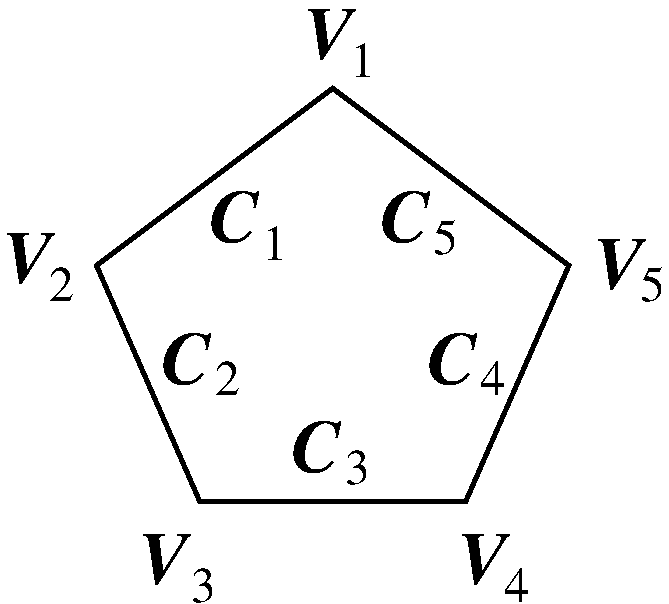
\includegraphics[width=4cm]{figures/pentagon.pdf}
	\caption{Vertex and chord labeling scheme for a pentagon, which coincides with the labeling scheme used by the pentagonal shape functions.}
	\label{figPentagon}
\end{figure}

\medskip\noindent
\textit{methods}

\medskip\noindent
\texttt{s = p.toString(state)}

\medskip\noindent
Returns a formatted string representation for this pentagon in configuration \texttt{state}.

\medskip\noindent
\texttt{n = p.number()}

\medskip\noindent
Returns the unique number affiliated with this pentagon.

\medskip\noindent
\texttt{n1, n2, n3, n4, n5 = p.chordNumbers()}

\medskip\noindent
Returns the chordal numbers associated with the chords of this pentagon, sorted from smallest to largest, i.e., not in accordance to Fig.~\ref{figPentagon}.

\medskip\noindent
\texttt{n1, n2, n3, n4, n5 = p.vertexNumbers()}

\medskip\noindent
Returns the vertex numbers associated with the vertices of this pentagon, sorted from smallest to largest, i.e., not in accordance to Fig.~\ref{figPentagon}.

\medskip\noindent
\texttt{truth = p.hasChord(number)}

\medskip\noindent
Returns \texttt{True} if one of the five chords has this chordal number; otherwise, it returns \texttt{False}.

\medskip\noindent
\texttt{truth = p.hasVertex(number)}

\medskip\noindent
Returns \texttt{True} if one of the five vertices has this vertex number; otherwise, it returns \texttt{False}.

\medskip\noindent
\texttt{c = p.getChord(number)}

\medskip\noindent
Returns the chord with specified \texttt{number}.  Typically called inside a \texttt{p.haschord if} clause.

\medskip\noindent
\texttt{v = p.getVertex(number)}

\medskip\noindent
Returns the vertex with specified \texttt{number}.  Typically called inside a \texttt{p.hasVertex if} clause.

\newpage
\medskip\noindent
\texttt{v = p.gaussPoints()}

\medskip\noindent
Returns the number of Gauss points associated with this pentagon.

\medskip\noindent
\texttt{p.update()}

\medskip\noindent
Establishes the fields that pertain to this object of class \texttt{pentagon} that affiliate with the next configuration.  It is to be called after all vertices and all chords have been updated.  This method does \textbf{not} call the \texttt{update} methods for the five vertices nor for the five chords that comprise this pentagon, but it does call the \texttt{update} methods for the \texttt{shapeFunction} and \texttt{membrane} objects contained within.  This method may be called multiple times before freezing its values with a call to \texttt{advance}.  (This method is called internally by \texttt{dodecahedron} objects.)

\medskip\noindent
\texttt{p.advance()}

\medskip\noindent
Assigns all of the object's data associated with the current configuration into their affiliated data associated with the previous configuration, and then assigns all of the object's data associated with the next configuration into their affiliated data associated with the current configuration, thereby freezing these data from external change.  This method does \textbf{not} call the \texttt{advance} methods for the five vertices nor for the five chords that make up this pentagon, but it does call the \texttt{advance} methods for the \texttt{shapeFunction} and \texttt{membrane} objects contained within.  (This method is called internally by \texttt{dodecahedron} objects.)

\medskip\noindent
\textit{The geometric fields associated with a pentagonal surface embedded in 3 space.}

\medskip\noindent
\texttt{a = p.area(state)}

\medskip\noindent
Returns the area of this irregular pentagon in configuration \texttt{state}.

\medskip\noindent
\texttt{aLambda = p.arealStretch(state)}

\medskip\noindent
Returns the square root of the area at \texttt{state} divided by reference area, i.e., $\sqrt{A / A_0}$.

\medskip\noindent
\texttt{aStrain = p.arealStrain(state)}

\medskip\noindent
Returns the logarithm of areal stretch evaluated at 'state', i.e., $\ln \sqrt{A / A_0}$.

\medskip\noindent
\texttt{daStrain = p.dArealStrain(state)}

\medskip\noindent
Returns the rate of areal strain at 'state', viz., $\tfrac{1}{2} A^{-1} \, \mathrm{d} A$.

\medskip\noindent
\texttt{[nx, ny, nz] = p.normal(state)}

\medskip\noindent
Returns the outward unit normal vector to this pentagon in configuration \texttt{state}.

\medskip\noindent
\texttt{[dnx, dny, dnz] = p.dNormal(state)}

\medskip\noindent
Returns the rate-of-change of the outward unit normal vector to this pentagon in configuration \texttt{state}.

\newpage
\medskip\noindent
\textit{Kinematic vector fields associated with the centroid of a pentagon in 3 space.}

\medskip\noindent
\texttt{[cx, cy, cz] = p.centroid(state)}

\medskip\noindent
Returns the centroid of this irregular pentagon in configuration \texttt{state}, i.e., this is vector $\boldsymbol{\chi}$ in Fig.~\ref{figPentagonCoord}.

\medskip\noindent
\texttt{[ux, uy, uz] = p.displacement(state)}

\medskip\noindent
Returns the displacement vector of its centroid in configuration \texttt{state}.

\medskip\noindent
\texttt{[vx, vy, vz] = p.velocity(state)}

\medskip\noindent
Returns the velocity vector of its centroid in configuration \texttt{state}.

\medskip\noindent
\texttt{[ax, ay, az] = p.acceleration(state)}

\medskip\noindent
Returns the acceleration vector of its centroid in configuration \texttt{state}.

\medskip\noindent
\textit{The rotation and spin of a pentagonal surface as it moves through 3 space.}

\medskip\noindent
\texttt{pMtx = p.rotation(state)}

\medskip\noindent
Returns a 3$\times$3 orthogonal matrix $\mathbfsf{P}$ that rotates the base vectors from its dodecahedral frame of reference into a set of local base vectors pertaining to this irregular pentagon whose outward normal aligns with the 3~direction, i.e., the irregular pentagon resides in the local pentagonal 1-2 plane.  The local 1~direction connects the shoulders of the pentagon, while the 2~direction is rooted at the head of the pentagon.  The returned matrix associates with configuration \texttt{state}.

\medskip\noindent
\texttt{omegaMtx = p.spin(state)}

\medskip\noindent
Returns a 3$\times$3 skew symmetric matrix $\boldsymbol{\Omega} \defeq \mathrm{d} \mathbfsf{P} \, \mathbfsf{P}^{\mathsf{T}}$ that describes the time rate of
rotation, i.e., a spin of the local pentagonal co-ordinate system about the
fixed co-ordinate system of its dodecahedron.  The returned matrix associates with configuration \texttt{state}.

\medskip\noindent
\textit{The kinematic tensor fields of a planar membrane evaluated in the reference co-ordinate system of the pentagon.  To rotate a tensor field from the pentagonal frame, say $\bar{\mathbfsf{A}}$, into its dodecahedral frame producing $\mathbfsf{A}$, apply the following map: $\mathbfsf{A} = \mathbfsf{P} \bar{\mathbfsf{A}} \mathbfsf{P}^{\mathsf{T}}$ where $\mathbfsf{P}$ is the orthogonal matrix returned by\/} \texttt{rotation}.

\medskip\noindent
\texttt{fMtx = p.F(gaussPt, state)}

\medskip\noindent
Returns the 2$\times$2 planar deformation gradient $\mathbfsf{F}$ located at \texttt{gaussPt} in configuration \texttt{state}.

\medskip\noindent
\texttt{dFdX = p.dFdX(gaussPt, state)}

\medskip\noindent
Returns the partial derivative taken with respect to the X direction of a 2$\times$2 planar deformation gradient, viz., $\mathbfsf{F}_{,1}$, located at \texttt{gaussPt} in configuration \texttt{state}.

\medskip\noindent
\texttt{dFdY = p.dFdY(gaussPt, state)}

\medskip\noindent
Returns the partial derivative taken with respect to the Y direction of a 2$\times$2 planar deformation gradient, viz., $\mathbfsf{F}_{,2}$, located at \texttt{gaussPt} in configuration \texttt{state}.

\newpage
\medskip\noindent
\texttt{gMtx = p.G(gaussPt, state)}

\medskip\noindent
Returns the 2$\times$2 planar displacement gradient $\mathbfsf{G}$ located at \texttt{gaussPt} in configuration \texttt{state}.

\medskip\noindent
\texttt{qMtx = p.Q(gaussPt, state)}

\medskip\noindent
Returns the 2$\times$2 re-indexing matrix $\mathbfsf{Q}$ located at \texttt{gaussPt} in configuration \texttt{state}.

\medskip\noindent
\texttt{rMtx = p.R(gaussPt, state)}

\medskip\noindent
Returns the 2$\times$2 rotation matrix $\mathbfsf{R}$ derived from a \textbf{QR} decomposition of the re-indexed deformation gradient, denoted as $\mathbfsf{R}\hspace{1pt}\boldsymbol{\mathcal{U}}$, located at \texttt{gaussPt} in configuration \texttt{state}.

\medskip\noindent
\texttt{uMtx = p.U(gaussPt, state)}

\medskip\noindent
Returns the 2$\times$2 Laplace stretch $\boldsymbol{\mathcal{U}}$ derived from a \textbf{QR} decomposition of the re-indexed deformation gradient located at \texttt{gaussPt} in configuration \texttt{state}.

\medskip\noindent
\texttt{uInvMtx = p.UInv(gaussPt, state)}

\medskip\noindent
Returns the inverse of a 2$\times$2 Laplace stretch $\boldsymbol{\mathcal{U}}^{-1}$ derived from a \textbf{QR} decomposition of the re-indexed deformation gradient located at \texttt{gaussPt} in configuration \texttt{state}.

\medskip\noindent
\texttt{duMtx = p.dU(gaussPt, state)}

\medskip\noindent
Returns a differential change in the 2$\times$2 Laplace stretch $\boldsymbol{\mathcal{U}}$ derived from a \textbf{QR} decomposition of the re-indexed deformation gradient located at \texttt{gaussPt} in configuration \texttt{state}.

\medskip\noindent
\texttt{duInvMtx = p.dUInv(gaussPt, state)}

\medskip\noindent
Returns a differential change in the inverse of a 2$\times$2 Laplace stretch $\boldsymbol{\mathcal{U}}^{-1}$ derived from a \textbf{QR} decomposition of the re-indexed deformation gradient located at \texttt{gaussPt} in configuration \texttt{state}.

\medskip\noindent
\textit{Scalar attributes that are extensive thermodynamic variables, and their rates.}

\medskip\noindent
\texttt{xi = p.dilation(gaussPt, state)}

\medskip\noindent
Returns the planar dilation derived from a \textbf{QR} decomposition of the re-indexed deformation gradient located at \texttt{gaussPt} in configuration \texttt{state}, i.e., $\xi = \ln \sqrt{ab/a_0b_0}$.

\medskip\noindent
\texttt{epsilon = p.squeeze(gaussPt, state)}

\medskip\noindent
Returns the planar squeeze derived from a \textbf{QR} decomposition of the re-indexed deformation gradient located at \texttt{gaussPt} in configuration \texttt{state}, i.e., $\varepsilon = \ln \sqrt{ab_0/a_0b}$.

\medskip\noindent
\texttt{gamma = p.shear(gaussPt, state)}

\medskip\noindent
Returns the planar shear derived from a \textbf{QR} decomposition of the re-indexed deformation gradient located at \texttt{gaussPt} in configuration \texttt{state}.

\medskip\noindent
\texttt{dDelta = p.dDilation(gaussPt, state)}

\medskip\noindent
Returns differential change in the dilation of an irregular pentagon located at \texttt{gaussPt} in configuration \texttt{state}.

\newpage
\medskip\noindent
\texttt{dEpsilon = p.dSqueeze(gaussPt, state)}

\medskip\noindent
Returns differential change in the squeeze of an irregular pentagon located at \texttt{gaussPt} in configuration \texttt{state}.

\medskip\noindent
\texttt{dGamma = p.dGamma(gaussPt, state)}

\medskip\noindent
Returns differential change in the shear of an irregular pentagon located at \texttt{gaussPt} in configuration \texttt{state}.
